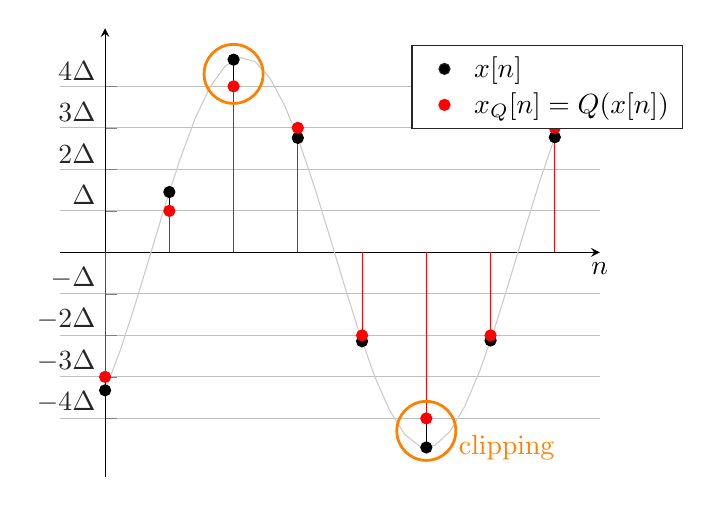
\begin{tikzpicture} 
\begin{axis}[
axis lines*=middle,
enlargelimits = true,
ymin=-4.5, ymax=4.5,
xmin=0, xmax=7,
axis line style={->,>=stealth},
xlabel={$n$},
yticklabel style = {yshift=0.2cm},
xticklabel style = {yshift=-0.1cm},
every axis x label/.style={
    at={(ticklabel* cs:1)},
    anchor=north,
},
every axis y label/.style={
    at={(ticklabel* cs:1)},
    anchor=south,
},
xtick=\empty,
ytick={-4,...,4},
yticklabels={$-4\Delta$,$-3\Delta$, $-2\Delta$, $-\Delta$, 0, $\Delta$, $2\Delta$, $3\Delta$, $4\Delta$},
every outer x axis line/.append style={white!15!black},
every x tick label/.append style={font=\color{white!15!black}},
ymajorgrids,
every outer y axis line/.append style={white!15!black},
every y tick label/.append style={font=\color{white!15!black}},
legend style={draw=white!15!black,fill=white,legend cell align=left, at={(axis cs: 9, 5)}}]

\addplot[black!20, domain=0:7, samples=31, forget plot] {4.7*cos(1.1*deg(x)-135)};
\addplot[ycomb, mark=*, domain=0:7, samples=8] {4.7*cos(1.1*deg(x)-135)}; \addlegendentry{$x[n]$};
\only<2-|handout:1>{
\addplot[ycomb, red, mark=*, domain=0:7, samples=8] {round(4.5*cos(1.1*deg(x)-135))}; \addlegendentry{$x_Q[n] = Q(x[n])$};

\node[draw=orange, circle, minimum size=0.75cm, line width=1pt] at (axis cs: 2, 4.3) {};
\node[draw=orange, circle, minimum size=0.75cm, line width=1pt] (c2) at (axis cs: 5, -4.3) {};
\node at (axis cs: 6.25, -4.7) {\color{orange} clipping};
}
\end{axis}
\end{tikzpicture}
